\chapter{短文本的视觉表达}

在我们的对话系统中,我们希望通过相似的视觉表达来关联相似的Post(帖子)。在早几年的微博中,对帖子(微博)的长度做了限制,最长不超过140个词。在样例帖子集(Sampled Post,我们在语料库中随机选取了34个帖子作为样例帖子集)中单词数量最高的帖子达到了58个词,这并不适合现在标签化的图片搜索引擎。一般来说,一段短文本单词数目越多,他表达的含义越丰富,也就越难用一个图像完整细致的表达。在分割的尝试过程中,我们也体会到了这种规律。

\begin{figure}[ht]
\centering
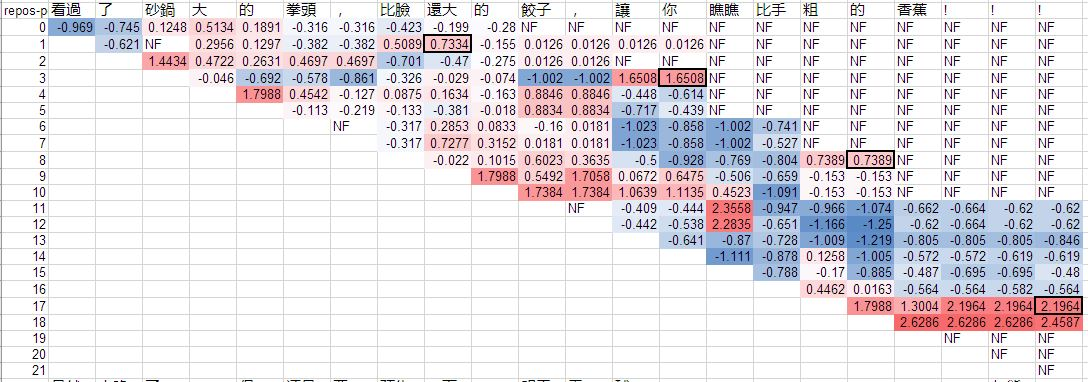
\includegraphics[width=14cm]{example_splitpost}
\caption{帖子的全切割视觉表达预测热力图} \label{fig:example_splitpost}
\end{figure}

如图\ref{fig:example_splitpost}是一个样例帖子分词后全分割尝试后的对其查询进行是否能视觉表达预测后的热力图。表格中第i行第j列,P$_{i,j}$ 代表着 Query$_{i,j}$的在视觉表达分类器中预测的结果,Query$_{i,j}$ 是帖子分词后第i个单词到第j个单词的子帖子,作为一个查询。比如第1行第4个数字 P$_{0,3}$ 为0.513356,代表着查询“看過了砂鍋大”能否视觉表达的可能性。图中$P_{i,j}$数值越大,颜色越红表示Query$_{i,j}$能视觉表达的可能性越大,反之颜色越蓝表示不能视觉表达的概率越大。在视觉分类器中将0作为分割线,P$_{i,j}$为正数表示其能视觉表达,P$_{i,j}$为负数表示它不能视觉表达。Query$_{i,j}$为NF(not found)表示查询没有搜索到图片,在样例中我们能观察到“NF”集中在右上角。这说明查询的长度越大,图片搜索引擎找到图片的可能性越小。因此我们很有必要对帖子做一些分割,使其能够更好的视觉表达。

我们想通过将帖子进行合理分割,使其变成的能视觉表达的帖子集。我们在图\ref{fig:example_splitpost}观察到,当查询长度稍短一些时,更容易视觉表达,但也会因此与句子意思偏离。我们还是想让查询在保存帖子原意的情况下,让查询能够视觉表达。我们尝试了许多种方法发现:\textbf{长度、标点符号、分词、去停顿词}都是合理的分割手段。考虑到顺序切割的末尾部分,我们都对尾部做了向前填充处理。

\section{独立分割}

\subsection{基于长度的分割}

在常识和实验中都表明了短文本的长度对其视觉表达有直接的影响。我们将帖子只基于长度的分割且不重复的分割成查询集,N代表了Query的长度。下面是详细的算法\ref{algo:SplitbyN}
\begin{algorithm}[htbp]
\SetAlgoLined
\KwData{Post,N}
\KwResult{Query[]}

initialization\;
\While{i < Post.length }{
    \eIf{i+N < Post.length}{
        Query[k]=Post.substr(i,i+N)\;
    }{
        Query[k]=Post.substr(Post.length-N,Post.length)\;
    }
	k++\;i+=N\;
}
\caption{SplitbyN}
\label{algo:SplitbyN}
\end{algorithm}
	
\subsection{基于分词的长度分割}
我们在研究样例帖子集的时候,发现只基于长度分割的会对产生很多错误分割,比如“阿森纳”是一个著名的足球俱乐部名称,但是如果长度恰好分割到之间,比如分为“阿森”和“纳”则与句子原语义产生较大的偏离。于是我们规定句子分离成分最小单位是单词而不是字,并按其最大字数N将其分离。具体算法详见\ref{algo:JiebaMN},算法主要是将词序列拼凑成尽可能接近于字数N的查询。并考虑了尾部补全和单词长度大于字数要求的情况,比如”中华人民共和国”。
\begin{algorithm}[htbp]
\SetAlgoLined
\KwData{PostWords[](Split by Jieba),N}
\KwResult{Query[]}

initialization\;
\While{i < PostWords.Count() }{
	j=0\;
	Query[k]=NULL\;
	\While{ i<PostWords.Count() and Query[k].length+PostWords[i].length<=N }{
		Query[k]+=PostWords[i]\;
		i++\; 
		}
    \If{i == PostWords.Count() }{
		Query[k]=NULL\;
		i--\;
		\While{i>=0 and Query[k].length+PostWords[i].length<=N}{
			Query[k]+=PostWords[i]\;
			i--\;
		}
		i=PostWords.Count()\;
	}
	\If{ i<PostWords.Count() and j==0 and Spost[i].length>N}{
		Query[k]=PostWords[i]\;
		i++\;
	}
	k++\;
}
\caption{JiebaMN}
\label{algo:JiebaMN}
\end{algorithm}

算法名称来自于我们所使用的分词算法,结巴(Jieba)分词。结巴分词号称做最好的Python中文分词组件。结巴中文分词采用的算法大致可以分为三个部分:首先基于Trie树结构高效地将词图扫描,生成句子中汉字所有可能成词情况,并由此构成一个有向无环图;然后利用动态规划查找最大概率路径, 找出基于词频的最大切分组合;最后对于未出现过的词,采用了基于汉字成词能力的HMM模型,使用了Viterbi算法。目前结巴分词支持三种分词模型:精确模式、全模式、和搜索引擎模式。我们使用了精确模式将我们的帖子分成了单词序列。

\subsection{基于标点的长度分割}
我们发现标点符号可以对其进行天然的语义分割,但是在我们的对话系统中,不是所有的标点都适合作为语义分割。比如书名号可以强调一本书名,但是如果将其强制作为语义分割符号,剩下的语义部分将会不完整。换句话说,有些标点符号会将帖子变成更小的语义单元,这几乎等同于中文分词。但是在较长的短文本中,我们还是希望将语义分割成相互独立的段落。一些断句所用的标点符号才是我们希望的使用的分割标识,比如句号、分号、问号、感叹号等。具体的分割算法件算法\ref{algo:SymbolMN}
\begin{algorithm}[htbp]
\SetAlgoLined
\KwData{PostWords[](Split by Jieba),N,SymbolSet}
\KwResult{Query[]}

initialization\;
\While{i < PostWords.Count() }{
	\eIf{(i == PostWords.Count() or PostWords[i] in SymbolSet) and (Query[k]!=NULL) }{
		k++\;
		Query[k]=NULL\;
	}{
		\If {Query[k].length+PostWords[i]>N and Query[k]!=NULL }{ 
			k++\;
			Query[k]=NULL \;
		}
		Query[k]+=PostWords[i]\;
	}
	i++;
}
\caption{SymbolMN}
\label{algo:SymbolMN}
\end{algorithm}

\subsection{实验数据}

我们对上述分割算法和长度都进行了尝试,并将其查询集经过自动检索的方法搜到的图片进行了人工标记,如图\ref{fig:post_quest}。与图\ref{fig:quest_vision}单词的视觉表达想对应的是,我们添加了一个问题“Query(查询)表达的意思是否符合Post(帖子)”来判断分割成子帖子之后的语义变化。

\begin{figure}[ht]
\centering
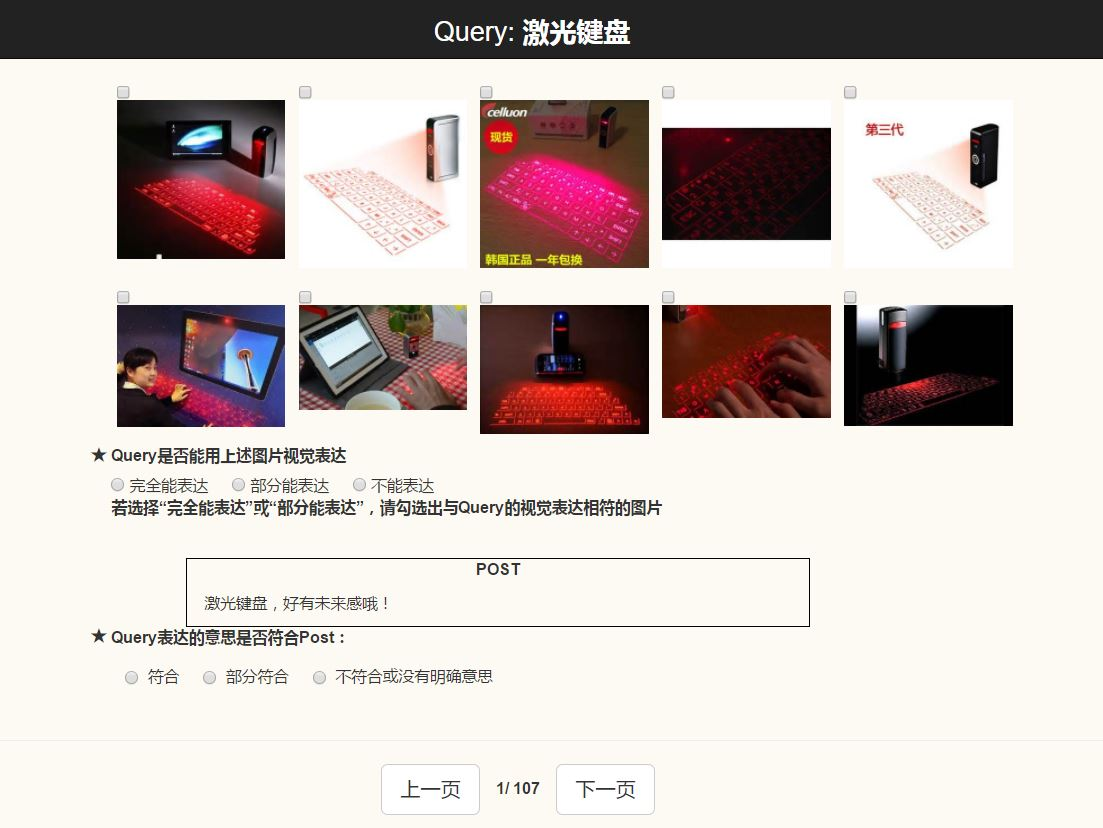
\includegraphics[width=14cm]{post_quest}
\caption{帖子视觉表达问卷调查} \label{fig:post_quest}
\end{figure}

如表\ref{tab:poem_result}所示,我们分析一些标记结果。我们在调查问卷中的问题“Query(查询)是否能够用图片视觉表达”中的选项,A:不能视觉表达标记为0分;B:部分能视觉表达标记为1分;C:能视觉表达标记为2分。归一化后算得如下表中的Wquery得分。同样的我们将问题“Query(查询)表达的意思是否符合Post(帖子)”选项,A:不符合Post标记为0分,B:部分符合Post标记为1分,C:符合Post标记为2分。归一化后算得如下表Wpost中得分。将两个分数相乘为Wq*Wq得分。在(a)表中Wpost参数中我们能清晰的发现查询字数和帖子原意的表达直接相关。Splitby10和Splitby12有大于10\%查询不返回图片,明显的高于其他方法。因此在人工标记后我们认为JiebaM8是独立分割方法中最能视觉表达的分割算法。
从人工标记的结果来看,短文本的视觉表达还是远不如单词的视觉表达。然而从表(a)中的结果来看,我们不能因为追求视觉表达而与原始帖子产生偏离。
\begin{table}[htp]
\centering
\caption{词视觉表达调查问卷结果} \label{tab:poem_result}
\begin{tabular}{ |c|c|c|c|}
    \hline
		查询集 & Wquery得分 & Wpost得分 & Wq*Wp得分 \\
	\hline
		Splitby4 &  0.5 & 0.372146 & 0.221461 \\ 
	\hline
		Splitby8 &  0.5 & 0.565789 & 0.291667 \\
	\hline
		Splitby12 & 0.45 & 0.725 &  0.298701  \\
 	\hline
\end{tabular}
\note{词视觉表达调查问卷结果(a)}
\begin{tabular}{ |c|c|c|c|}
    \hline
		查询集 & Wquery得分 & Wpost得分 & Wq*Wp得分 \\
	\hline
		Splitby6 &  0.24 & 0.35 & 0.156667 \\ 
	\hline
		Splitby8 &  0.276316 & 0.346491 & 0.157895 \\
	\hline
		Splitby10 & 0.3535 & 0.378788 &  0. 209596 \\
 	\hline
\end{tabular}
\note{词视觉表达调查问卷结果(b)}
\begin{tabular}{ |c|c|c|c|}
    \hline
		查询集 & Wquery得分 & Wpost得分 & Wq*Wp得分 \\
	\hline
		JiebaM8 &  0.401709 & 0.487179 & 0.373932 \\ 
	\hline
		Splitby8 &  0.355263 & 0.416667 & 0.322368 \\
	\hline
		SymbolM8 & 0.3375 & 0.391667 &  0.35625 \\
 	\hline
\end{tabular}
\note{词视觉表达调查问卷结果(C)}
\end{table}



\section{关联分割}

人在理解一个帖子,并对其产生回复的时候很多时候并不需要对其产生很全面的回复,可能就是几个关键词。在我们最开始的例子“创新工场三年庆,在我们的「智慧树」会议室。”评论都是针一个或几个方面展开。其中的关键词并不是相互独立的,我们可以对“创新工场、年庆”产生回复,也能对"年庆 会议室”产生回复。

我们将帖子结巴分词后,使用simHash算法过滤掉停顿词,剩下的单词作为标签,进行WxCy组合。WxCy组合是指,每x个关键词(标签),重复y个。我们使用视觉表达分类器后预测统计如下表\ref{tab:pred_WxCy}

\begin{table}[htbp]
\centering
\caption{WxCy视觉表达预测统计} \label{tab:pred_WxCy}
\begin{tabular}{|c|c|c|c|c|c|c|c|}
    \hline
    funName	 & pre$_{+}$	& pre$_{-}$	 & pre$_{NF}$	& all	& pred$_{+}$\%	& pre$_{-}$\% & 	pre$_{NF}$\% \\
Sampled\_W3C1	& 44	& 139 &	3& 	186 &	0.236559	 & 0.747312	& 0.016129 \\ 
\hline
Sampled\_W3C2	& 128	& 228 &	5& 	361 &	0.354571	 & 0.621579	& 0.013850 \\ 
\hline
Sampled\_W4C1	& 29	& 83 &	8& 	120 &	0.241667	 & 0.691667	& 0.066667 \\ 
\hline
Sampled\_W4C2	& 43	& 124 &	8& 	175 &	0.245714	 & 0.708571	& 0.045714 \\ 
\hline
Sampled\_W5C1	& 17	& 64 &	4& 	85 &	0.200000	 & 0.752941	& 0.047059 \\ 
\hline
Sampled\_W5C2	& 18	& 88 &	7& 	113 &	0.159292	 & 0.778761	& 0.061947 \\ 
\hline
Sampled\_W6C1	& 19	& 43 &	3& 	65 &	0.292308	 & 0.661538	& 0.046154 \\ 
\hline
Sampled\_W6C2	& 14	& 60 &	3& 	77 &	0.181818	 & 0.779221	& 0.038961 \\ 
\hline
Sampled\_W7C1	& 9	& 37 &	5& 	51 &	0.176471	 & 0.725490	& 0.098039 \\ 
\hline
Sampled\_W7C2	& 14	& 39 &	7& 	60 &	0.233333	 & 0.650000	& 0.116667 \\ 
\hline
Sampled\_W8C1	& 17	& 19 &	8& 	44 &	0.386364	 & 0.431818	& 0.181818 \\ 
\hline
Sampled\_W8C2	& 19	& 22 &	9& 	50 &	0.380000	 & 0.440000	& 0.180000 \\ 
\hline
Sampled\_W9C1	& 11	& 12 &	9& 	32 &	0.343750	 & 0.375000	& 0.281250 \\ 
\hline
Sampled\_W9C2	& 14	& 11 &	9& 	34 &	0.411765	 & 0.323529	& 0.264706 \\ 
\hline

\end{tabular}
%\note{这里是表的注释}
\end{table}

在表中,pre$_{+}$表示视觉分类预测的值为正数即查询能视觉表达,pre$_{-}$表示视觉分类器预测的值为负数,pre$_{NF}$表示查询没有返回图片。在上表中W3C2和W6C1方法的查询集能视觉表达的概率更高且只有很小的概率搜索不到图片。

\section{对话系统}
我们将Splitby12、JiebaM8、W6C1、W3C2四种方法在对话系统中做了尝试。我们每个查询后取得的图片进行特征提取后变成一个256维的向量。我们将查询图片集的向量进行K-means聚类后取出最大类的中心作为查询的视觉表达。每个帖子被分割成一个查询集,通过查询集的视觉表达的来寻找相似的帖子。对话系统寻找评论的部分由李顶龙同学完成,这里只贴出跟我的方法选择相关的实验结果。

\begin{table}[htbp]
\centering
\caption{对话系统的人工标记结果} \label{tab:STC_result}
\begin{tabular}{ |c|c|c|c|}
    \hline
		方法 & image256 & image256-char256 & char256\\
	\hline 
		Splitby12 & 1.0067 & 1.058 & 1.0318 \\
	\hline 
		JiebaM8 & 1.0513 & 1.0407 & 1.0226  \\
	\hline
		W3C2 & 1.0067 & 1.125 & 1.0226  \\
	\hline 
		W6C1 & 1.0067 & 1.0208 & 1.0226\\
 	\hline
\end{tabular}
%\note{这里是表的注释}
\end{table}

如表\ref{tab:STC_result}所示的结果,image256表示单纯用图片关联相关帖子的结果,Char256表示用文字关联的结果,image256-char256表示两种方法的结合。表中的值是对话系统在测试帖子上提交的结果。虽然最高值在W3C2方法中的图像和文字方法中取得。总的来说,图片对文字关联方法只有微弱的提升。



